\documentclass[../Tesi.tex]{subfiles}


\begin{document}
\section{Progettazione}
	\subsection{Architettura ad alto livello}
		\begin{figure}[!h]
			\centering
			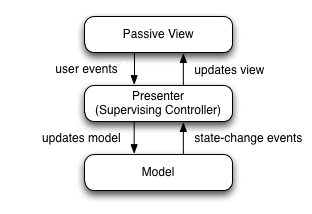
\includegraphics[scale=0.6]{images/mvp}
				\caption{Rappresentazione pattern MVP}
		\end{figure}

		L'architettura dell'applicazione segue il pattern architetturale Model-View-Presenter, utilizzato insieme alla dependency injection. Tale scelte, unite ad un uso diffuso di interfacce permettono di ridurre il grado di accoppiamento tra le parti che l'applicazione in modo tale da aumentarne il più possibile l'estensibilità.

		\paragraph*{Model}
		Il model rappresenta i dati che vengono trattati all'interno dell'applicazione. Le classe appartenenti al model rappresentano:
		\begin{itemize}
			\item i dati che vengono salvati in modo persistente nel database presente nel dispositivo in cui è installata l'applicazione;
			\item gli statement che devono essere inviati ad un LRS;
			\item gli oggetti che vengono scambiati tra JavaScript e Android per il tracciamento delle esperienze di un utente;
			\item oggetti che permettono l'accesso a tali dati.
		\end{itemize}
		Nell'applicativo è rappresentato dal package omonimo.

		\paragraph*{Presenter}
		Il presenter si occupa di recuperare i dati del model e passarli alla view per essere mostrati. Esso si occupa inoltre di gestire le richieste della view in seguito ad una interazione con un utente. \\ Nell'applicativo è rappresentato dal package omonimo.

		\paragraph*{View}
		La view si occupa della dell'interfaccia grafica dell'applicazione e di notificare al presenter le interazioni dell'utente, che ha il compito di elaborare. \\ Nell'applicativo è rappresentato dal package omonimo.
	
	\subsection{Persistenza dei dati}
		\subsubsection{Il database locale}
		L'applicazione si appoggia su di un database creato utilizzando la libreria Realm per il salvataggio dei dati relativi agli utenti, ai contenuti e alla loro fruizione in un database locale. In tale database, vengono salvati i dati relativi ai contenuti xAPI, che devono essere visualizzati, la prima volta che l'applicazione viene avviata, mentre i dati relativi all'utente vengono salvati quando viene effettuato un login o la registrazione. I dati di fruizione, invece, vengono registrati ad ogni interazione di un utente con una slide di un corso.
			
			\paragraph{Diagramma ER}
			\hfill \break
				\begin{figure} [H]
					\centering
					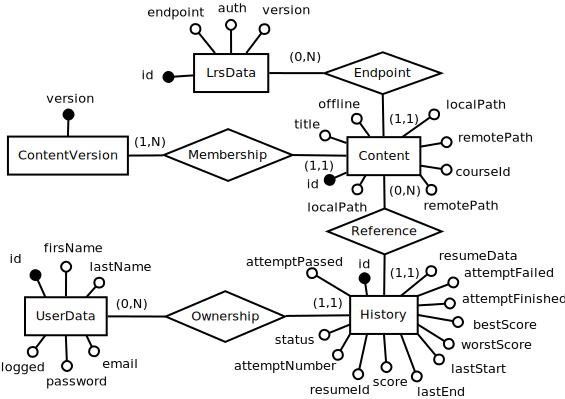
\includegraphics[scale=0.9]{images/er/RealmDB}
						\caption{Diagramma ER del database locale}
				\end{figure}

			\paragraph{Descrizione delle relazioni}
			\subparagraph*{Content}
			Relazione che contiene le informazioni dei contenuti xAPI che devono essere gestiti dall'applicazione. Attributi:
			\begin{itemize}
				\item \textbf{id}: chiave primaria, intero;
				\item \textbf{title}: stringa, rappresenta un titolo associato al contenuto;
				\item \textbf{remotePath}: stringa, rappresenta l'URL a cui è possibile recuperare il contenuto;
				\item \textbf{localPath}: stringa, rappresenta il percorso locale al dispositivo a cui è possibile recuperare il contenuto, se questo è disponibile offline;
				\item \textbf{offline}: boolean, indica se il contenuto è disponibile per la riproduzione offine oppure no;
				\item \textbf{courseId}: stringa, rappresenta l'identificativo utilizzato dal LRS per distinguere un contenuto;
				\item \textbf{lrsDataId}: intero, chiave esterna verso la relazione LrsData.
			\end{itemize}

				\subparagraph*{ContentVersion}
				Relazione che serve per specificare la versione dei contenuti trattati dall'applicazione. Attributi:
				\begin{itemize}
					\item \textbf{version}: chiave primaria, stringa, rappresenta la versione dei contenuti.
				\end{itemize}

				\subparagraph*{LrsData}
				Relazione che contiene le informazioni riguardanti un LRS a cui inviare i dati di fruizione dei contenuti di un certo utente. Attributi:
				\begin{itemize}
					\item \textbf{id}: chiave primaria, intero;
					\item \textbf{endpoint}: stringa, rappresenta l'URL a cui inviare gli statement in formato xAPI;
					\item \textbf{auth}: stringa, rappresenta metodo e dati per l'accesso al LRS;
					\item \textbf{version}: stringa, rappresenta la versione di statement xAPI accettata dal LRS.
				\end{itemize}

				\subparagraph*{History}
				Relazione che contiene i dati di fruizione di ogni contenuto per gli utenti che hanno utilizzato l'applicazione su di un determinato dispositivo. Attributi:
				\begin{itemize}
					\item \textbf{id}: chiave primaria, intero;
					\item \textbf{resumeId}: stringa, identificativo utilizzato dalla componente che si occupa della riproduzione dei contenuti xAPI per l'accesso ai dati per riprendere un contenuto da dove lo si aveva interrotto all'ultima fruizione;
					\item \textbf{resumeData}: stringa, dati per riprendere un contenuto da dove lo si aveva interrotto all'ultima fruizione;
					\item \textbf{status}: intero, rappresenta lo stato in cui si trova un contenuto per un certo utente. Può rappresentare che un utente non ha mai acceduto ad un certo contenuto, che vi ha acceduto ma il contenuto non è stato fruito fino alla fine oppure che un utente ha superato o meno un certo contenuto;
					\item \textbf{score}: double, rappresenta l'ultimo punteggio ottenuto da un utente per un certo contenuto;
					\item \textbf{bestScore}: double, rappresenta il miglior punteggio ottenuto da un utente per un certo contenuto;
					\item \textbf{worstScore}: double, rappresenta il peggior punteggio ottenuto da un utente per un certo contenuto;
					\item \textbf{lastStart}: long, timestamp in millisecondi dell'ultima volta che un utente ha iniziato un certo contenuto;
					\item \textbf{lastStart}: long, timestamp in millisecondi dell'ultima volta che un utente ha terminato un certo contenuto;
					\item \textbf{attemptNumber}: intero, rappresenta il numero di volte che un utente ha iniziato un certo contenuto;
					\item \textbf{attemptFinished}: intero, rappresenta il numero di volte che un utente ha terminato un certo contenuto;
					\item \textbf{attemptPassed}: intero, rappresenta il numero di volte che un utente ha superato un certo contenuto;
					\item \textbf{attemptFailed}: intero, rappresenta il numero di volte che un utente non ha superato un certo contenuto;
					\item \textbf{contentId}: intero, chiave esterna verso la relazione Content. Rappresenta il contenuto a cui fanno riferimento i dati;
					\item \textbf{userId}: intero, chiave esterna verso la relazione UserData. Rappresenta l'utente a cui fanno riferimento i dati.
				\end{itemize}

				\subparagraph*{UserData}
				Relazione che contiene le informazioni degli utenti che hanno utilizzato l'applicazione su di un determinato dispositivo. Attributi:
				\begin{itemize}
					\item \textbf{id}: chiave primaria, intero;
					\item \textbf{logged}: boolean, indica se un utente è loggato in quel dispositivo o meno;
					\item \textbf{email}: stringa, rappresenta l'email di un utente;
					\item \textbf{password}: stringa, rappresenta la password di un utente;
					\item \textbf{firstName}: stringa, rappresenta il nome di un utente;
					\item \textbf{lastName}: stringa, rappresenta il cognome di un utente.
				\end{itemize}

			\paragraph{Descrizione delle associazioni}
				\subparagraph*{Membership}
				Associazione che unisce ogni contenuto alla sua versione.\\
				\textbf{Molteplicità}:(1,N) ogni versione può essere associato a più contenuti, ogni contenuto può avere un'unica versione.

				\subparagraph*{Endpoint}
				Associazione che unisce ogni contenuto al LRS a cui devono essere inviati i dati di fruizione.\\
				\textbf{Molteplicità}:(1,N) ogni LrsData può essere associato a più contenuti, ogni contenuto si riferisce ad un unico LrsData.

				\subparagraph*{Reference}
				Associazione che unisce ogni contenuto ai dati di fruizione per un certo utente.\\
				\textbf{Molteplicità}:(1,N) ogni contenuto può essere associato a più History, ogni History può essere associata ad un solo contenuto.

				\subparagraph*{Ownership}
				Associazione che unisce ogni utente ai dati di fruizione di un certo contenuto.\\
				\textbf{Molteplicità}:(1,N) ogni utente può essere associato a più History, ogni History può appartenere ad un unico utente.

			\subsubsection{Specifica dei contenuti}
			I contenuti che l'applicazione deve gestire e di cui deve permettere l'accesso agli utenti vengono, come già accennato, vengono specificati in un file JSON che l'applicazione scarica. Tale scelta, anche se non ottimale, è stata fatta in previsione della creazione di un database che comprenda tutti i contenuti xAPI fruibili dall'applicazione. Infatti è possibile sostituire, nel file di configurazione dell'applicazione, l'indirizzo di tale file con una richiesta ad un server, il quale si occuperà di fornire all'applicazione i contenuti da mostrare agli utenti in un formato similare a quello del file attuale. Una volta effettuato il download di tale file, i contenuti al suo interno vengono utilizzati per riempire il database locale, in modo tale da potervi associare i dati di fruizione degli utenti.

			\subsubsection{Persistenza degli statement}
			Gli statement creati dall'applicazione per registrare i dati di fruizione dei contenuti xAPI sono salvati temporaneamente all'interno di un database SQLite, completamente gestito dalla libreria TinCanAndroid-Offline. Quando l'applicazione registra che è disponibile una connessione internet si occupa di inviare tali statement ad un LRS. Anche l'invio è gestito dalla libreria TinCanAndroid-Offline, che provvede, nel caso in cui non vi siano errori, ad eliminare dal database locale tutti gli statement inviati. Ad ogni avvio l'applicativo ha il compito di interrogare l'LRS a cui sono stati inviati i dati di fruizione al fine di verificare se vi siano dati che non sono presenti in locale: se presenti il database locale viene aggiornato. Poichè LRS utilizzato è Learning Locker, il quale utilizza come DBMS MongoDB, le richieste per recuperare dati dal LRS saranno delle query MongoDB e i risultati di tali richieste saranno in formato JSON.
				\paragraph{Struttura degli statement}
				Gli statement accettati da un LRS sono oggetti JSON che devono seguire la sintassi definita dalla specifica xAPI. Tali oggetti hanno alcuni campi obbligatori, altri opzionali che specificano le proprietà dello statement. In particolare, in questo progetto, i campi definiscono le azioni di uno specifico utente rispetto ad un determinato contenuto. Alcuni campi degli statement possono essere sia specificati da chi invia i dati, sia dal LRS che li riceve, altri invece devono essere inseriti o da un componente o dall'altro. Di seguito sono spiegati i campi utilizzati dagli statement inviati dall'applicazione.
					\subparagraph{ID}
					Il campo \textit{ID} identifica uno statement in modo univoco all'interno di un LRS. Tale campo può essere specificato dal LRS, qualora non sia stato inserito da chi invia lo statement. Deve essere un UUID.

					\subparagraph{actor}
					Il campo \textit{actor} identifica la persona o l'oggetto a cui è associato un determinato statement. Negli statement utilizzati dall'applicativo è un oggetto composto a sua volta dai campi:
					\begin{itemize}
						\item \textbf{name}: stringa che rappresenta un nome associato alla persona o oggetto a cui è riferito lo statement;
						\item \textbf{mbox}: stringa che rappresenta una email nella forma ``mailto:email address'' che serve per l'identificazione di un singolo utente; 
						\item \textbf{objectType}: attributo che serve per specificare che gli statement sono riferiti a singole persone o sistemi. Per questo, in tutti gli statement inviati dall'applicazione, tale campo sarà fissato uguale a ``Agent''.
					\end{itemize}
					Per l'identificazione degli utenti si è scelto di utilizzare il campo \textit{mbox} per semplicità di gestione. Infatti la specifica xAPI permette, per identificare un utente, di associargli un generico URI oppure di specificare un oggetto \textit{account}.

					\subparagraph{verb}
					Il campo \textit{verb} identifica l'azione compiuta dal soggetto specificato nel campo \textit{actor}. Tale campo è un oggetto composto a sua volta dai campi:
					\begin{itemize}
						\item \textbf{id}: stringa che rappresenta un IRI che contiene il significato del verbo;
						\item \textbf{display}: oggetto che permette di rappresentare il verbo in varie lingue.
					\end{itemize}
					I verbi utilizzati nell'applicazione e il loro \textit{id} fanno riferimento alla pagina \url{http://xapi.vocab.pub/datasets/adl/}, nella quale è presente una lista di verbi utilizzabili con gli statement xAPI.

					\subparagraph{object}
					Il campo \textit{object} specifica l'oggetto a cui è rivolto il verbo dichiarato nel campo \textit{verb}. Negli statement generati dall'applicazione questo campo è utilizzato per specificare o un contenuto o una slide specifica appartenente ad un contenuto. Tale campo è un oggetto composto a sua volta dai campi:
					\begin{itemize}
						\item \textbf{objectType}: stringa che rappresenta il tipo di oggetto. Deve essere sempre uguale a ``Activity se presente'';
						\item \textbf{id}: stringa che rappresenta un identificativo del contenuto o della slide, formattata come IRI;
						\item \textbf{definition}: serve per specificare nome e descrizione dell'oggetto in varie lingue, oltre a specificare di che tipo di oggetto si tratta.
					\end{itemize}

					\subparagraph{context}
					Il campo \textit{context} è un campo non obbligatorio che serve per specificare delle informazioni contestuali allo statement a cui appartiene. Questo campo, negli statement generati dall'applicazione, è sempre presente e specifica sempre il contenuto a cui si riferisce uno statement.

					\subparagraph{stored}
					Il campo \textit{stored} è un campo che indica il timestamp di quando è stato salvato lo statement da parte del LRS.

					\subparagraph{timestamp}
					Il campo \textit{timestamp} è un campo che indica il timestamp di quando è stata effettuata l'azione specificata dal campo \textit{verb} da parte di un utente.

			\subsubsection{Autenticazione e registrazione}
			L'autenticazione e la registrazione all'applicazione avvengono mediante delle richieste HTTP a due URL specificati nel file di configurazione dell'applicativo. Tale scelta è stata fatta per permettere di cambiare agevolmente tali indirizzi, senza dover modificare il codice. \\In fase di sviluppo sono stati creati anche due script PHP ed un database per gli utenti dell'applicazione. Tali script, raggiungibili agli indirizzi specificati nel file di configurazione, si occupano rispettivamente del login e della registrazione, interrogando il database degli utenti e restituendo il risultato della richiesta.

	\subsection{Comunicazione tra Javascript e Android}
	Al fine di tracciare le attività degli utenti sui contenuti xAPI è stato necessario creare sia in JavaScript che in Android delle componenti che si occupassero direttamente della comunicazione tra questi linguaggi. La parte JavaScript ha il compito di recuperare le informazioni di interazione degli utenti con i contenuti e loro invio all'applicazione Android. Quest'ultima si occupa di creare gli statement dai dati che riceve e del loro invio al LRS. Le informazioni vengono recuperate da un'altra componente JavaScript, chiamata \textit{player}, che si occupa della riproduzione dei contenuti xAPI, nei dispositivi mobili. Tale componente contiene delle variabili relative allo stato del contenuto in riproduzione, come il numero della slide, un eventuale punteggio dell'utente o quando è stato iniziato il contenuto, e si occupa di reagire all'interazione dell'utente o di mostrare la sequenza delle slide in un determinato ordine. 
	È stato creato quindi uno script che ascolta il cambiamenti della variabile del \textit{player} che si occupa delle slide visitate da un utente e, ad ogni variazione, raccoglie un insieme di dati e li invia all'applicazione Android. Quest'ultima si occupa di trasformare quanto ricevuto in statement. Tutto ciò è possibile riproducendo i contenuti xAPI in una \textit{WebView} a cui è aggiunta una \textit{JavaScriptInterface}, la quale espone dei metodi che possono essere invocati dalla componente JavaScript che si occupa del recupero delle informazioni. I dati passati tra Android e JavaScript sono degli oggetti in formato JSON.

\end{document}